\section{Biot-Savart Law Exercises With Current Loops}
\begin{comment}
This lab was written by Ted Bunn for spring of 2016.  It was edited slightly by Matt Trawick for this manual in April 2016.

\end{comment}

\makelabheader %(Space for student name, etc., defined in master.tex)

\bigskip

\textbf{Activity 1: Magnetic Field Above a Current Loop}

We have a horizontal 
circular current loop of radius $R$, carrying
current $I$.  We want to determine the magnetic field at a point $P$ a
height $z$ directly above the center of the loop.
The pictures below show the situation.  In the edge-on view shown on the right, 
the $\vv{ds}_1$ and $\vv{ds}_2$ are current elements (small segments of the current loop) perpendicular
to the page.

\vskip 0.4in
\begin{center}
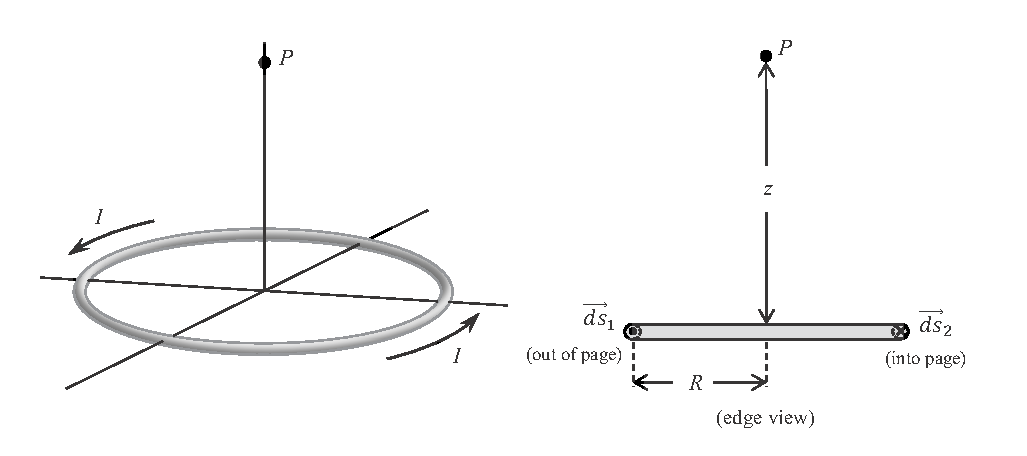
\includegraphics{biot_savart_above_loops/circular_loop_3d.eps}
\end{center}

%\begin{enumerate}[leftmargin=0in, labelwidth=*, align=left, labelsep=0in, widest=a, itemindent=\labelwidth, label=(\emph{\alph*})]
\begin{enumerate}[wide, label=(\emph{\alph*})]
\item On the edge-view diagram above, draw the direction of the vector $\vv{dB}_1$,
which is the magnetic field produced by the current element $\vv{ds}_1$.  Put the
tail of the vector at the point $P$, the place where the field
is being evaluated.  

\item \label{mag}
Use the Biot-Savart law to express the magnitude of $\vv{dB}_1$
in terms of the various given quantities in the problem such as $ds$, $I$,
$R$, and $z$.
\answerspace{0.7in}

\item Now consider the current element $\vv{ds}_2$ on the exact opposite
side of the loop.  Draw the direction of the magnetic field $\vv{dB}_2$
caused by this current element.  (Label your vectors $\vv{dB}_1$ and $\vv{dB}_2$ 
to distinguish them)

\item When we eventually add up (i.e., integrate) all the $\vv{dB}$'s from
all the different current elements, what will be the direction of  
the resulting
vector?
\answerspace{0.5in}

\item \label{component}
Before we do the integration, we need to pick out just that
one component of $\vv{dB}$.  Indicate an appropriate angle $\theta$
on your drawing, and write down an expression giving the
relevent component of $\vv{dB}$ in terms of the magnitude
$dB$ and the angle $\theta$.
\answerspace{0.5in}

\item \label{triangle}
We need to express the angle $\theta$ in terms of the given
quantities in the problem.  In order to do this, identify a right
triangle containing $\theta$ and also the dimensions $R$ and $z$.  Use this triangle
to express the relevant trigonometric function of $\theta$
in terms of $R$ and $z$.  
\answerspace{0.5in}

\item Put your answers to questions \ref{mag}, \ref{component},
\ref{triangle} together
to give an expression giving the relevant component of $\vv{dB}$
in terms of the various given quantities $I$, $R$, $z$, and $ds$.
\answerspace{0.5in}

\item \label{answer1}
Integrate the previous expression to get the magnitude of the
magnetic field produced by the entire loop of current.  (Note: if you
find yourself doing a hard integral, you're thinking about it the wrong
way!)
\answerspace{1in}

\item What does your answer say about the strength of the magnetic
field right at the center of the loop, at the point $z=0$?
(The result should agree with the expression we got earlier for 
this quantity, namely $B=\mu_0I/2R$.)
\answerspace{0.5in}

\end{enumerate}

\bigskip

{\bf Activity 2: Magnetic Field Above a Square Loop}

Now suppose that we have a loop of wire shaped like a square as shown.
The square lies in the $xy$ plane and is centered on the origin.
Each side has length $2a$, so that it extends from $-a$ to $a$.
It carries current $I$ going counterclockwise.  As in the previous
part, our goal is to calculate the magnetic field at a point 
located a height $z$ above the center of the loop.  

\vspace{0.4in}
\centerline{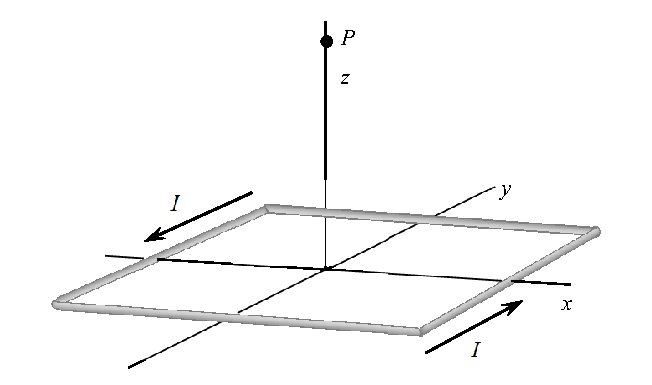
\includegraphics{biot_savart_above_loops/square_loop_3d.eps}}
\medskip


To do this, we'll have to consider one side of the square at a time.  In
each case, we'll want to know the magnetic field produced by 
a straight segment of current.  Fortunately, you worked out
that expression in Lab \ref{biot_savart_straight_wire}. 


Let's start by considering 
the side on the left of the picture, which extends from
$(x,y)=(-a,-a)$ to $(x,y)=(-a,+a)$.

\begin{enumerate}[wide, label=(\emph{\alph*})]

\item Draw an arrow on the figure indicating the 
direction of the magnetic field due to this segment.
Call it $\vec{B}_1$.

\item The magnitude of $\vec{B}_1$ is given by the formula
you derived in Lab \ref{biot_savart_straight_wire}. What is it? Note: the thing
called $y$ in that lab is the distance from the center of
the wire to the point at which the field is being evaluated. 
In this case, what is that quantity (in terms of $z$ and $a$)?
\answerspace{0.7in}

\item When we add up the contributions from all four sides, only
one component is going to matter.  Decide which
component that is. Then indicate an
appropriate angle $\theta$ on your drawing, and 
write down an expression giving
the magnitude of the relevant component of $\vec{B}_1$ in terms of $\theta$.  
\answerspace{0.7in}

\item Draw a triangle showing the angle $\theta$ from the previous part,
as well as lengths such as $z$ and $a$.  Express the relevant trigonometric
function of $\theta$ in terms of these quantities.
\answerspace{0.7in}

\item Put the last three steps together to get an expression giving the
relevant component of $\vec{B}_1$ in terms of the given quantities of the
problem, such as $I$, $a$, and $z$.  
\answerspace{0.7in}

\item \label{answer2}
The other three sides of the square will give contributions
$\vec{B}_2,\vec{B}_3,\vec{B}_4$ to the magnetic field.  When you add
up all four sides, what will the resulting magnetic field be?
This is the final answer to the question we originally posed.
\answerspace{0.7in}

\item What is the strength of the magnetic field right at the
center of the square (that is, at $z=0$)?
\answerspace{0.7in}

\end{enumerate}

\pagebreak[2]
\textbf{Activity 3: The Field at Very Great Distances}

In this activity, we'll consider the results of the previous
two calculations in the case where $z$ is very large -- that is,
the case where we're very far away from the current loop.

\begin{enumerate}[wide, label=(\emph{\alph*})]

\item Take your expression from question \ref{answer1} of Activity 1,
giving the magnetic field above a circular current loop.
Suppose that we're extremely far away from the loop, that is,
that $z$ is much, much greater than $R$.  In that case, we can approximate
$z^2+R^2\approx z^2$.  Write down the expression for the magnetic
field strength in this approximation.  
\answerspace{0.7in}

\item Your answer to the previous question should have $R$'s in it.
For reasons that we'll see in a minute, it turns out to be nice
to express the answer in terms of the area $A$ of the loop instead of the
radius.  Make the appropriate substitution to get an expression
giving $B$ in terms of $I,A,z$.
\answerspace{0.7in}

Next, we'll play the same game with the square loop.  

\item Using your expression from question \ref{answer2} of Part 2,
write down an approximate expression for $B$ assuming that the distance
$z$ is very large.
\answerspace{0.7in}

\item What is the area of the square loop (in terms of $a$)?  
Express the answer to the previous question in terms of the area $A$
instead of the length $a$.
\answerspace{0.7in}

\end{enumerate}

You should find that the expressions are the same for the circular
and square loops.  (If you did not find this, talk to me.)
This result turns out to be true for loops of all shapes: as long as you're
far away from the loop, the magnetic field depends on the area of the loop,
but not on its exact shape.


